%%%%%%%%%%%%%%%%%%%%%%%VICARIOUS%%%%%%%%%%%%%%%%%%%%%%%%%%%%%%%%%%%%%%%
% 																	%
% Template for presentation in Latex`s Beamer Class					%
% Using the default Berlin theme, can be replaced by other themes		%
% logo in the upper right can be replaced by new .png, gif, eps etc	%
% 																	%
%%%%%%%%%%%%%%%%%%%%%%%%%%%%%%%%%%%%%%%%%%%%%%%%%%%%%%%%%%%%%%%%%%%%%%%
\documentclass[xcolor=dvipsnames, aspectratio=169]{beamer}
\usetheme{Berlin}
\usecolortheme[named=LimeGreen]{structure}
\usepackage{beamerthemesplit} % kam neu dazu
\usepackage[ngerman]	{babel}			
\usepackage{t1enc}						
\usepackage[utf8]{inputenc}			
\usepackage{amsmath}
\usepackage{graphicx}
\graphicspath{{pictures/}}
\usepackage{amssymb}
\usepackage{amsfonts}
\usepackage{caption}
\usepackage{multimedia}
\usepackage{tikz}
\usepackage{listings}
\usepackage{acronym}
\usepackage{subfig}

\usepackage{lmodern}
\usepackage{multicol}

\definecolor{pblue}{rgb}{0.13,0.13,1}
\definecolor{pgreen}{rgb}{0,0.5,0}
\definecolor{pred}{rgb}{0.9,0,0}
\definecolor{pgrey}{rgb}{0.46,0.45,0.48}

\lstset{
    escapeinside={(*}{*)}
}

\lstdefinestyle{Java}{
  showspaces=false,
  showtabs=false,
  tabsize=2,
  breaklines=true,
  showstringspaces=false,
  breakatwhitespace=true,
  commentstyle=\color{pgreen},
  keywordstyle=\color{pblue},
  stringstyle=\color{pred},
  basicstyle=\footnotesize\ttfamily,
  numbers=left,
  numberstyle=\tiny\color{gray}\ttfamily,
  numbersep=7pt,
  %moredelim=[il][\textcolor{pgrey}]{$$},
  moredelim=[is][\textcolor{pgrey}]{\%\%}{\%\%},
  captionpos=b
}

\lstdefinestyle{basic}{  
  basicstyle=\footnotesize\ttfamily,
  breaklines=true
  numbers=left,
  numberstyle=\tiny\color{gray}\ttfamily,
  numbersep=7pt,
  backgroundcolor=\color{white},
  showspaces=false,
  showstringspaces=false,
  showtabs=false,
  frame=single,
  rulecolor=\color{black},
  captionpos=b,
  keywordstyle=\color{blue}\bf,
  commentstyle=\color{gray},
  stringstyle=\color{green},
  keywordstyle={[2]\color{red}\bf},
}


\lstdefinelanguage{custom}
{
morekeywords={public, void},
sensitive=false,
morecomment=[l]{//},
morecomment=[s]{/*}{*/},
morestring=[b]",
}


\lstdefinestyle{BashInputStyle}{
  language=bash,
  showstringspaces=false,
  basicstyle=\small\sffamily,
  numbers=left,
  numberstyle=\tiny,
  numbersep=5pt,
  frame=trlb,
  columns=fullflexible,
  backgroundcolor=\color{gray!20},
  linewidth=0.9\linewidth,
  xleftmargin=0.1\linewidth
}

%Logo in the upper right just change if you know what you are doing^^
\addtobeamertemplate{frametitle}{}{%
\begin{tikzpicture}[remember picture,overlay]
\node[anchor=north east,yshift=2pt] at (current page.north east) {
\includegraphics[height=1.8cm]{htw}};
\end{tikzpicture}}

\begin{document}
\bibliographystyle{alpha}
\title{Netzwerke -- Übung SoSe 2019}
\subtitle{Vorschau: Einfache Netzwerke\\
		\href{mailto:Benjamin.Troester@HTW-Berlin.de}{Benjamin.Troester@HTW-Berlin.de}\\
		PGP: ADE1 3997 3D5D B25D 3F8F 0A51 A03A 3A24 978D D673 }

\author{Benjamin Tröster}

\date{}

\begin{frame}
\titlepage

\end{frame}

\section*{Road-Map}
\begin{frame}
\frametitle{Road-Map}
\begin{multicols}{2}
  \tableofcontents
\end{multicols}
\end{frame}

\section{Netzwerke -- Grundlagen}
\begin{frame}
	\frametitle{Was ist ein Netzwerk}
	\begin{columns}
		\begin{column}{0.5\textwidth}
   			\begin{itemize}
   				\item Netzwerk besteht im wesentlichen aus drei Komponenten
   				\item Endsysteme -- senden \& empfangen Daten
   				\item Zwischenknoten -- leiten Daten weiter
   				\item Links/Verbindungen -- verbinden Endsysteme \& Zwischenknoten
   			\end{itemize}
		\end{column}
	\begin{column}{0.5\textwidth}  %%<--- here
	\begin{figure}
    \begin{center}
     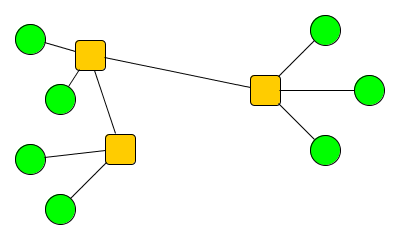
\includegraphics[width=0.8\textwidth]{network}
     \caption{Netzwerk: Grün Endsysteme, gelb Zwischenknoten, Kanten als Links}
     \end{center}
     \end{figure}
\end{column}
\end{columns}
\end{frame}

\begin{frame}
	\frametitle{Endknoten}
	\begin{figure}
		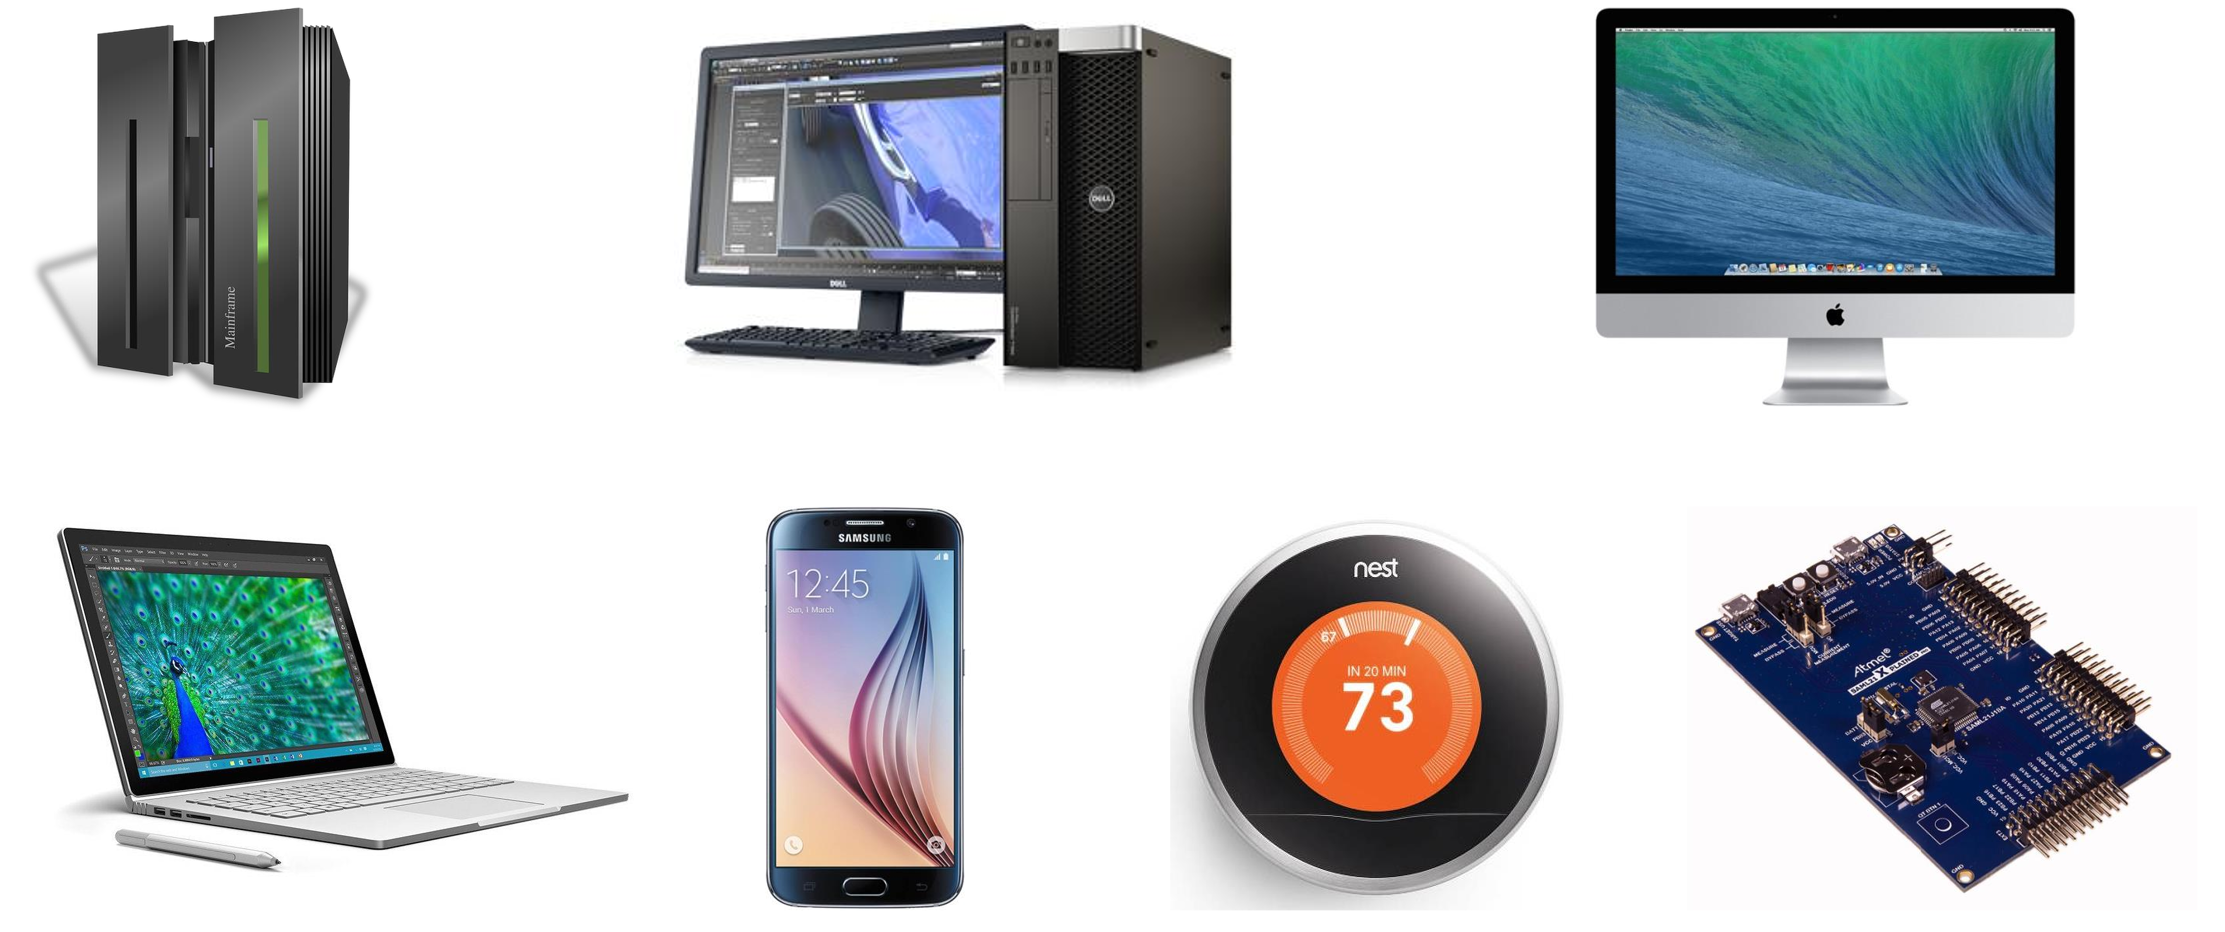
\includegraphics[scale=0.15]{endknoten}
	\end{figure}
\end{frame}

\begin{frame}
	\frametitle{Zwischenknoten}
	\begin{figure}
		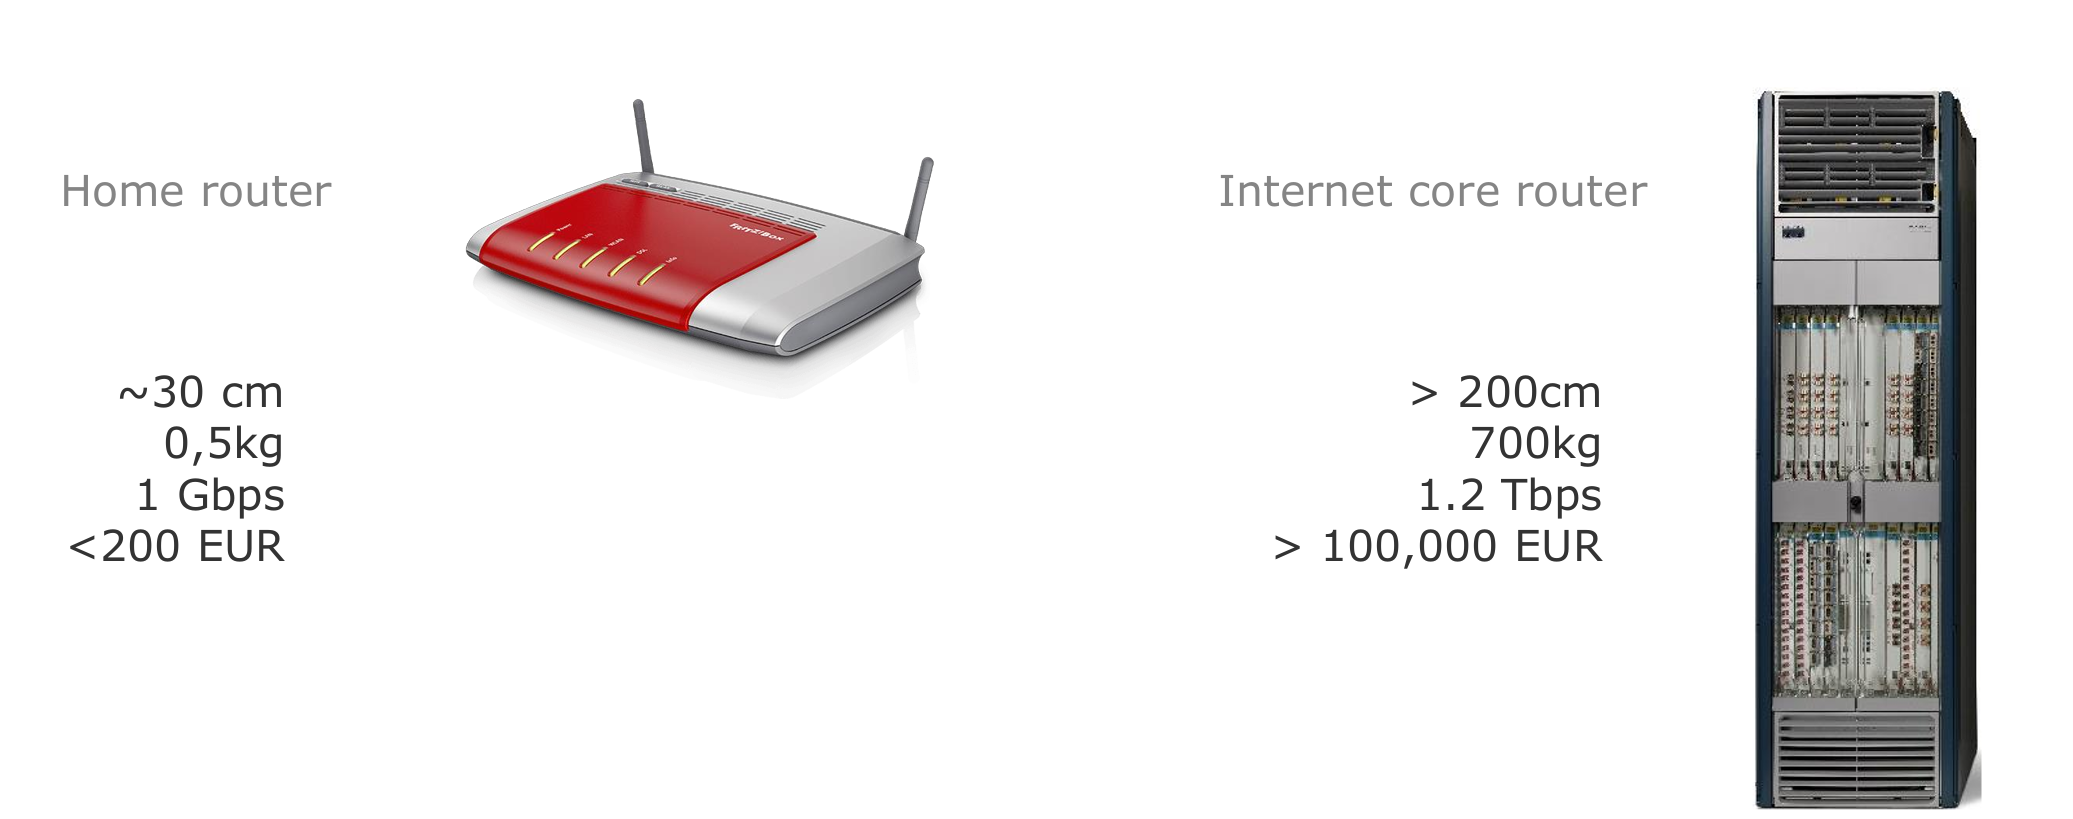
\includegraphics[scale=0.15]{zwischenknoten}
	\end{figure}
\end{frame}

\begin{frame}
	\frametitle{Links}
	\begin{figure}
		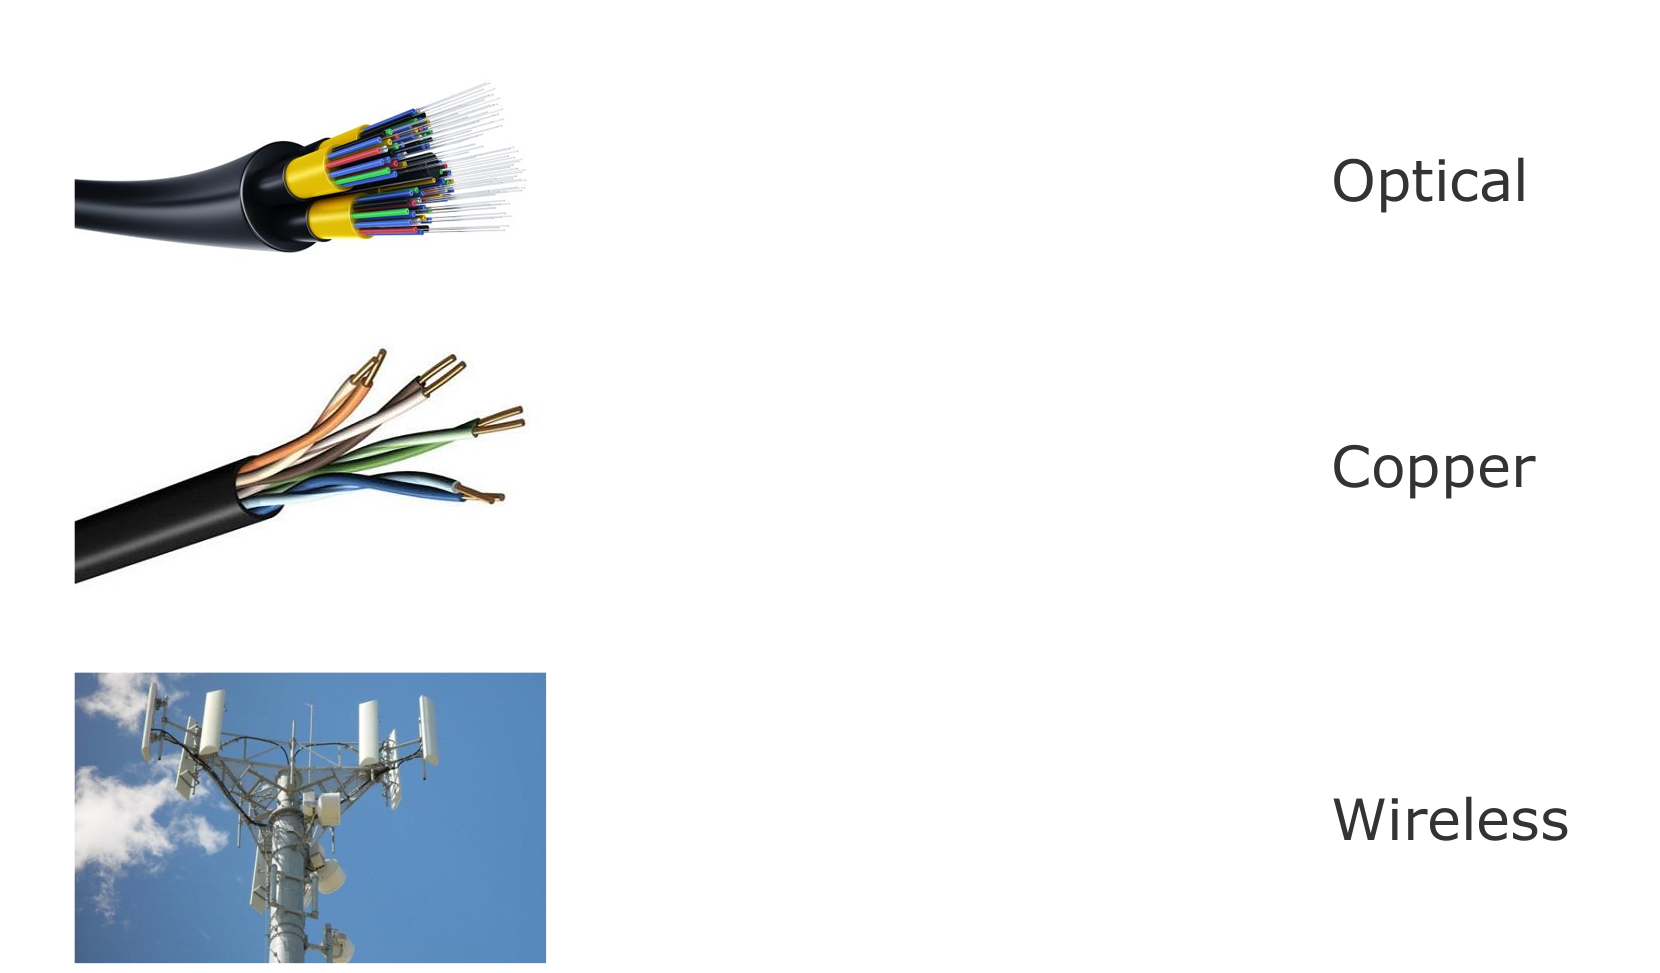
\includegraphics[scale=0.15]{links}
	\end{figure}
\end{frame}

\section{Netzwerktopologien}
\begin{frame}
	\frametitle{Netzwerktopologien}
	\begin{itemize}
		\item Netzwerktopologie beschreibt, wie die Knoten einander erreichen könnten
		\item Drei wesentliche Anforderung an die Topologie:
		\begin{itemize}
			\item Fehlertoleranz -- mehre Pfade zwischen Quelle und Ziel
			\item Ausreichende Teilung, sodass Top. praktikabel \& kosteneffizient ist -- Anzahl der Links sollte nicht zu hoch sein
			\item Sollte ausreichend pro Knoten Kapazität bereitstellen -- Anzahl der Links sollte nicht zu klein sein
		\end{itemize}
	\end{itemize}
\end{frame}

\begin{frame}
	\frametitle{Beispieltopologien}
	\begin{figure}
	\center
		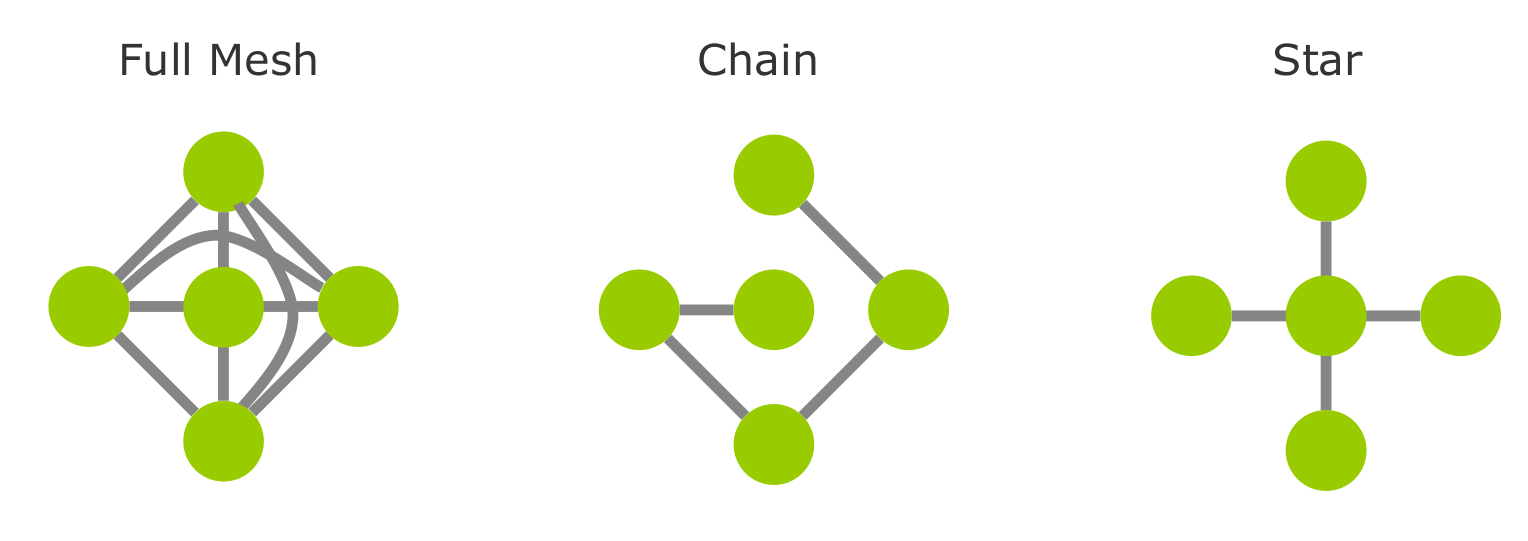
\includegraphics[scale=0.20]{topologie}
	\end{figure}
	\begin{itemize}
		\item Vorteile:
		\item Nachteile:
	\end{itemize}
\end{frame}

\section{OSI-Modell}
\begin{frame}
	\frametitle{OSI-Modell}
	Netzwerkkommunikation kann in sieben Schichten (Layer) zerlegt werden \footnote{Informatiker lieben Schichtenmodelle und Modularisierung!}
	\begin{columns}
		\begin{column}{0.5\textwidth}
   			\begin{itemize}
   				\item Für die nächsten Übungen wichtig:
   				\begin{enumerate}
   					\item Physical Layer
   					\item Data Link Layer
   					\item Network Layer
   					\item Transport Layer
   				\end{enumerate}
   			\end{itemize}
		\end{column}
	\begin{column}{0.5\textwidth}
	\vspace{-1cm}
	\begin{figure}
    \begin{center}
     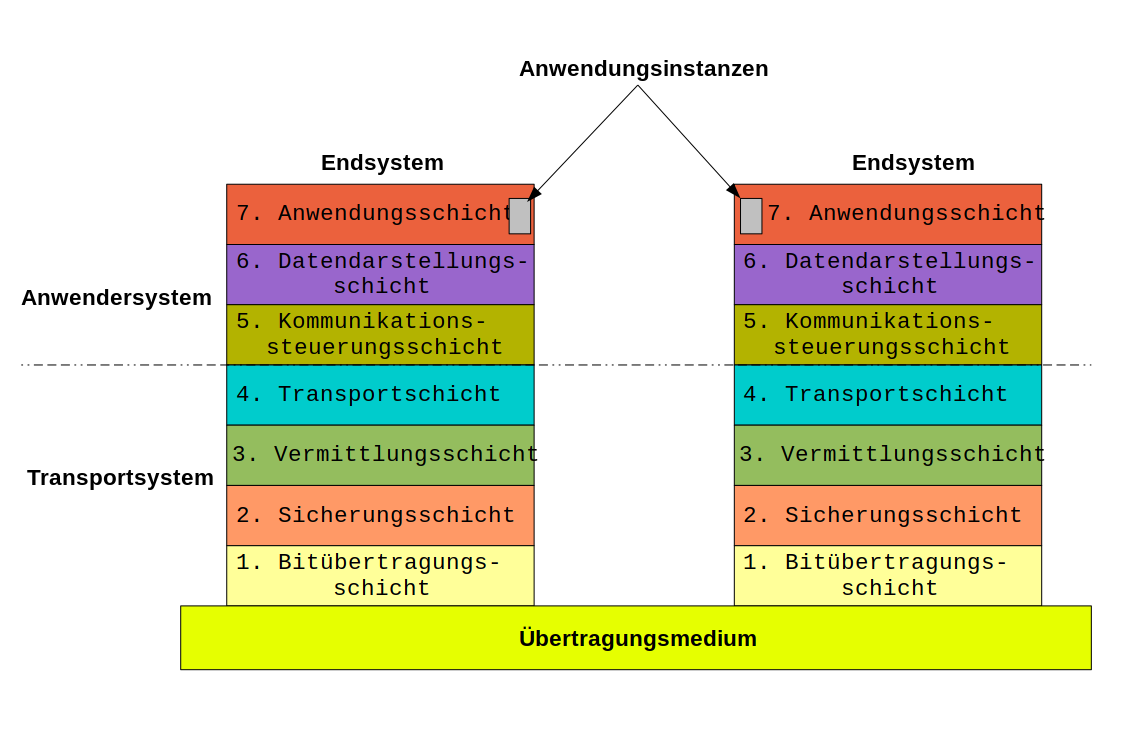
\includegraphics[scale=0.2]{osi_modell}
     \end{center}
     \end{figure}
\end{column}
\end{columns}
\end{frame}

\section{Laborhardware}
\subsection{Raspberry Pi}
\begin{frame}
	\frametitle{Raspberry Pi}
 \hspace*{-1cm}
\begin{minipage}{0.7\textwidth}
\begin{itemize}
	\item Raspberry Pi 3 Model B
	\item Architektur: ARM Cortex(64-Bit) Broadcom BCM2837
	\item Quad Core 4 $\times$ ARM Cortex-A53 @ 1.2GHz
	\item 1GB LPDDR2 (900 MHz)
	\item 10/100 Ethernet, 2.4GHz 802.11n wireless
	\item 4 USB 2 ports
	\item Raspbian 9 Stretch -- Debian Fork
\end{itemize}
\end{minipage}%
\begin{minipage}{0.3\textwidth}
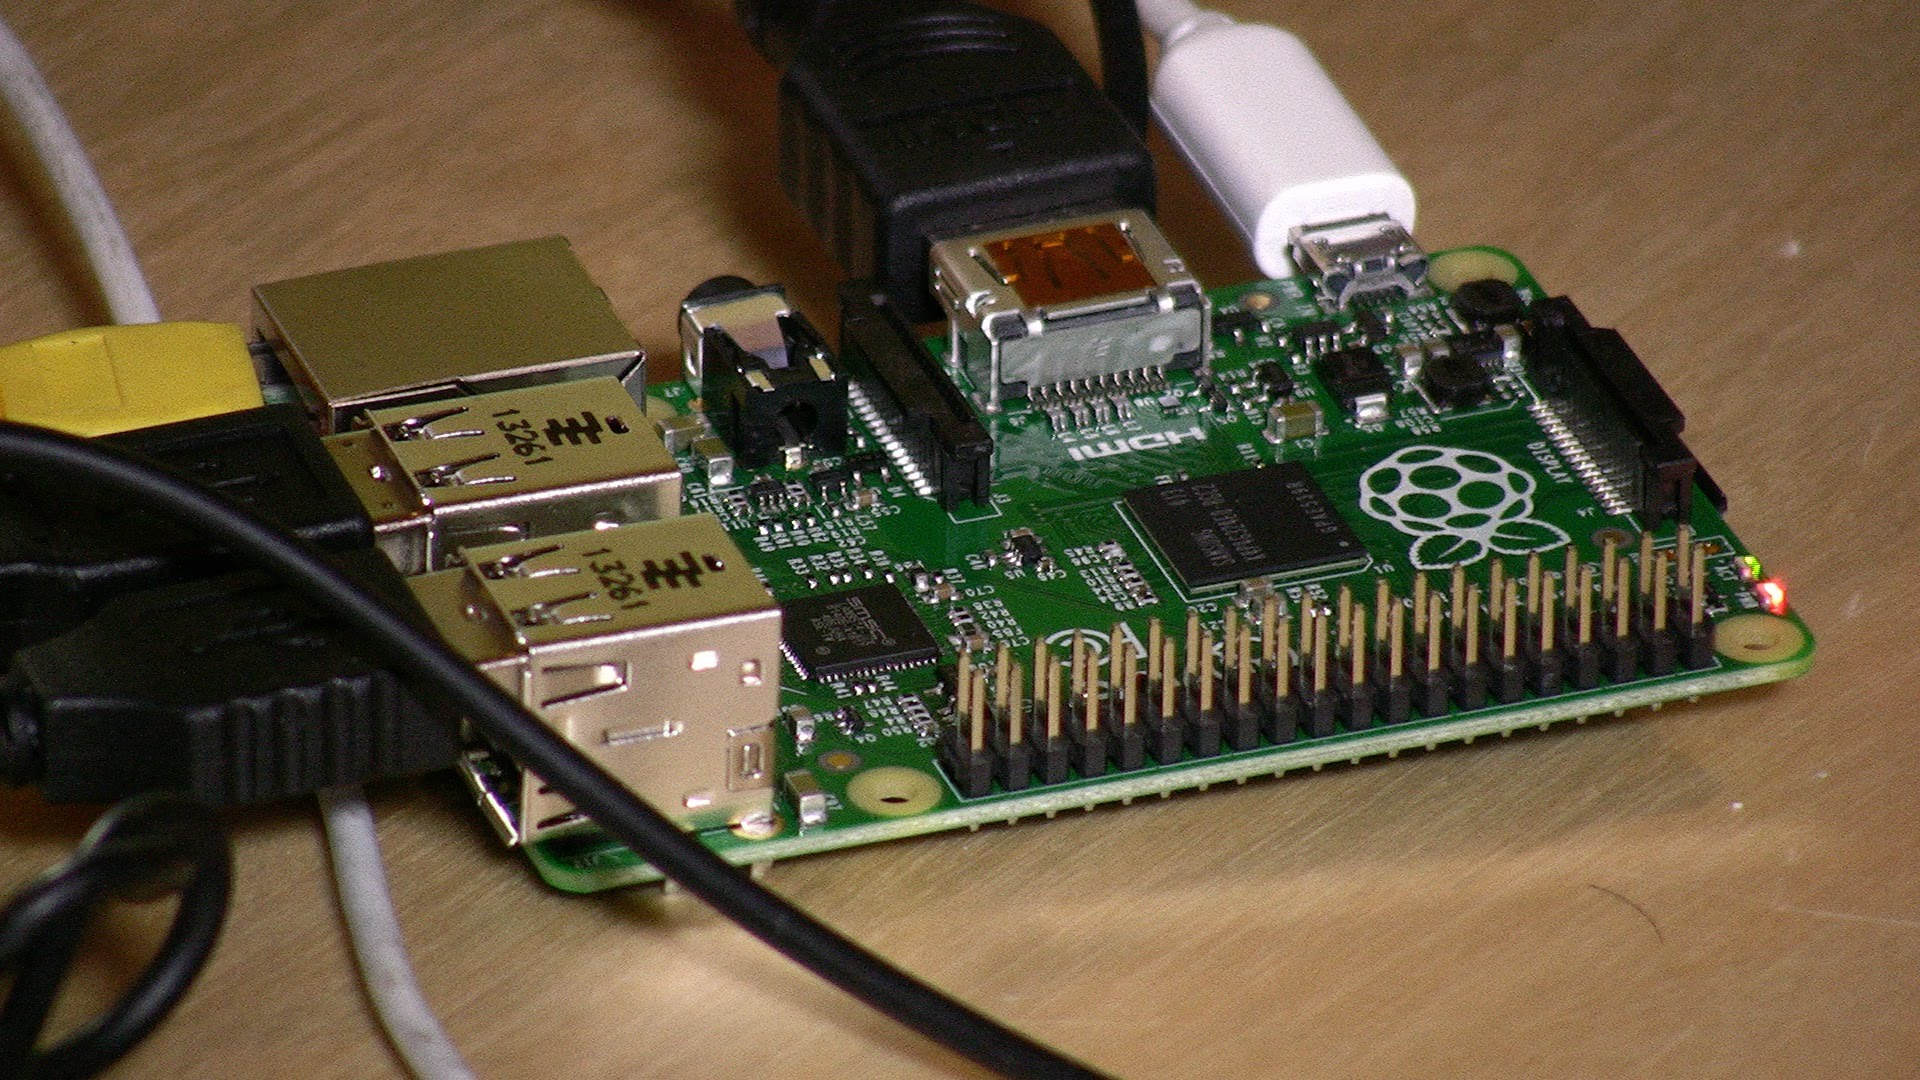
\includegraphics[scale=0.06]{raspi}
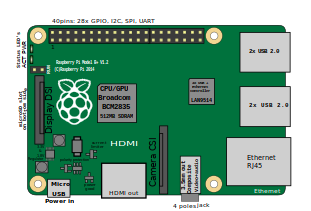
\includegraphics[scale=0.45]{raspib1+}
\end{minipage}\hfill
\end{frame}

\subsection{Switch}
\begin{frame}
	\frametitle{Switch}
	\begin{columns}
		\begin{column}{0.5\textwidth}
   			\begin{itemize}
   				\item 8 Port 100 Mbit Switch
   				\begin{itemize}
   					\item Sollte auf jedem Tisch liegen
   					\item Zwischenknoten -- leitet den Verkehr zwischen den Endknoten weiter 
   					\item Arbeitet auf OSI-Layer 2 -- kennt kein IP nur Ethernet-Frames \& MAC-Adressen
   					\item Switches sind über den Switch im Rack miteinander verbunden
   					\item Uplink ins Internet 1 Gbit symmetrisch -- ebenfalls im Rack 
   				\end{itemize}
   			\end{itemize}
		\end{column}
	\begin{column}{0.5\textwidth}  %%<--- here
	\vspace{-1cm}
	\begin{figure}
    \begin{center}
     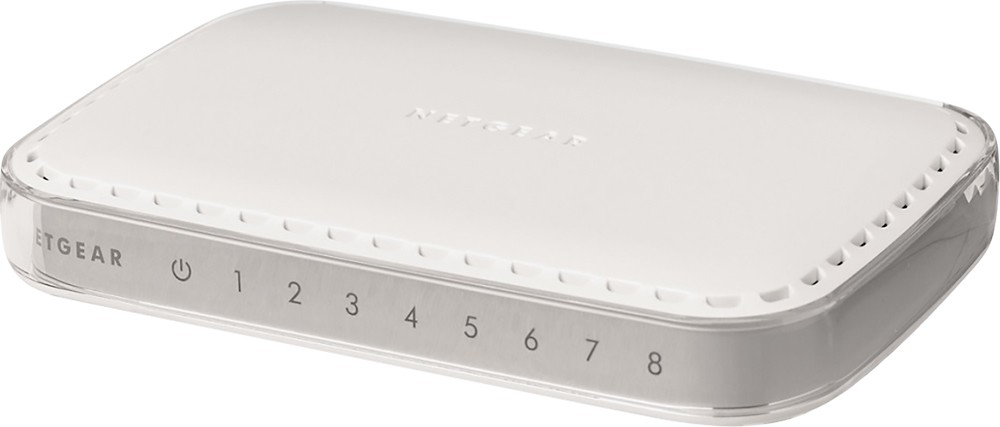
\includegraphics[scale=0.2]{netgear_switch}
     \end{center}
     \end{figure}
\end{column}
\end{columns}
\end{frame}

\begin{frame}
	\frametitle{19$"$ Server Rack}
	\begin{columns}
		\begin{column}{0.5\textwidth}
	\begin{itemize}
		\item Uplink ins DFN
		\item Switch für das Labornetzwerk
		\item Router aus dem Labornetzwerk
		\item Cisco Router für Backbone Routing
		\item MoCo-Cloud für Big Data Arbeitsgruppe
	\end{itemize}
	\end{column}
	\begin{column}{0.5\textwidth}  %%<--- here
	\vspace{-1cm}
\begin{figure}%
    \centering
	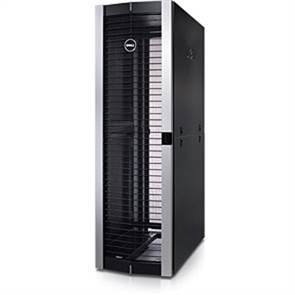
\includegraphics[scale=0.5]{dell}
\end{figure}
\end{column}
\end{columns}
\end{frame}

\section{Empfehlungen}
\begin{frame}{Nerd-Wochenmarkt}
Empfehlung der Woche:
\begin{itemize}
	\item n00bCore:
	\begin{itemize}
		\item \glqq n00bfreundlicher Podcast über Computer\grqq
		\item \url{http://n00bcore.de/nc-006-was-ist-ein-internet/}
	 	\item \url{http://n00bcore.de/nc007-away/} 
	\end{itemize}
	\item Freifunk Rheinland RoutingDays 2016
	\begin{itemize}
		\item \url{https://media.ccc.de/b/conferences/routingdays/routingdays16}
		\item Speziell: \url{https://media.ccc.de/v/routingdays16-18-network_ip_basics}
	\end{itemize}
\end{itemize}
\end{frame}


\end{document}